\section{Data}\label{sec:data}
\setstretch{1.5}

Table \ref{table:stats} presents summary statistics at the baseline year for all the variables used in this analysis: variables related to the EC/29, fiscal data, health inputs, infant mortality rates, birth outcomes, and control variables.

\subsection{EC/29 and Fiscal Data}

To evaluate municipalities' fiscal reactions to the EC/29, we combine public spending data from the Brazilian Finance System (FINBRA)\footnote{All spending data is presented in 2010 R\$. We used the General Price Index (IGP) to correct values}, which covers the period of 1998 to 2010, with data from the Brazilian National System of Public Health Budget (Datasus/SIOPS)\footnote{SIOPS was created right after the EC/29 to monitor revenues and expenditure in the provision of health care at the state and municipal levels, and to monitor compliance with the EC/29.} available from 2000 onward. FINBRA provides data on total public spending, and spending by a few aggregated categories, such as Health and Sanitation, Education and Culture, etc, and data on public revenues. The SIOPS, on the other hand, provides more detailed information on public health spending, which allow us to evaluate how municipalities allocate resources within the public health sector. It gathers data on total health spending, health spending from own resources, health spending from intergovernmental transfers, and health spending by types of spending, including spending in human resources, investments, services from third parties, and others\footnote{Others expenditures includes mainly administrative spending}. Moreover, SIOPS calculates for each municipality the share of own resources spent in the provision of health care, that we use to build our independent variable.

Figure \ref{fig:5} displays the spatial variation in the share of own resources spent in health. Municipalities below the EC/29 are represented with colors in the red scale, while municipalities above the target are represented with the blue scale. The map shows significant differences in the share of own resources spent in health within the same state, providing the identifying variation of this study as we include state fixed-effects in our main specification. 

\begin{figure}[h!]
\begin{center}
    \caption{EC/29 Compliance Geographic Variation}
    \scalebox{0.7}{
    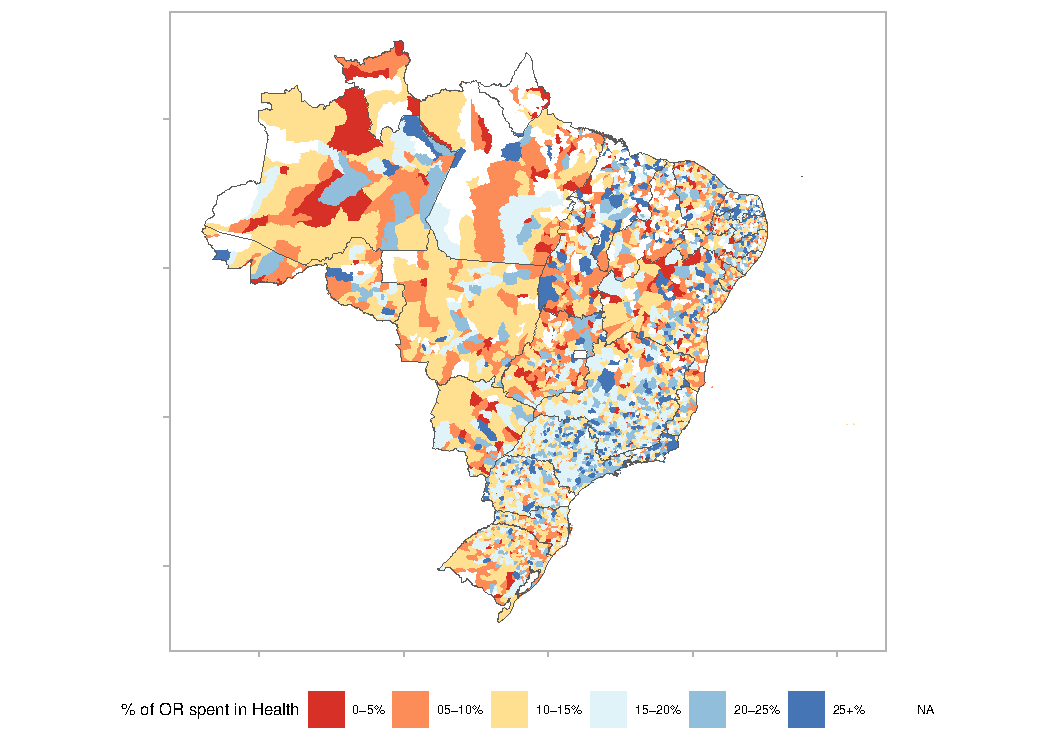
\includegraphics{plots/ec29_map.pdf}
    \label{fig:5}
    }
\end{center}
\end{figure}

\subsection{Health Inputs}

We combine data from several sources to build our health inputs data base. First we collect data on primary care coverage - extensive and intensive margin -  from Brazilian National System of Information on Primary Care (Datasus/SIAB) . Data on health human resources and hospital infrastructure comes from the 1999, 2002, 2005 and 2009 Medical-Sanitary Assistance Survey (AMS), a census of the health sector run by Brazilian Institute of Geography and Statistics (IBGE). 

The Brazilian National System of Information on Ambulatory Care (Datasus/SIA) every ambulatory procedure funded by SUS, with information on the type and complexity of the procedure, the health professional responsible, and the corresponding health facility register number. This data is used to create variables on ambulatory production, primary care ambulatory production, and ambulatory production by procedures complexity. We also use this data to indirectly create variables that measure the supply of health ambulatory facilities, as well as the supply of ambulatory facilities with health professionals related to primary care services. This is done by evaluating the number of facilities within a municipality that recorded ambulatory procedures of interests or ambulatory procedures executed by specific professionals of interest \footnote{We are able to construct these variables only for the period of 1998 to 2007, as changes in the SIA classification of ambulatorial procedures changes in 2008.}.

To measure access to health services, we used data from the from Brazilian National System of Birth Records (Datasus/SINASC), that records every birth in Brazil and provides detailed information on these births. Using this data we calculated the share of no prenatal visits, 1-6 prenatal visits and more than 7 prenatal visits. Importantly, in the first years of our sample, there is no information on prenatal visits for a considerable amount of births. To account for this under-registration issue, we also calculated the share of prenatal ignored. By estimating the impacts on this variable, we can separate the effects of access increasing from improvements in data registration.


\subsection{Infant Mortality and Birth Outcomes}

We use micro-data from Brazilian National System of Mortality Records (Datasus/SIM) and from SINASC to construct Infant Mortality Rates. These micro-data allow us to construct Infant Mortality Rates by the timing of death, and for the main causes of death. Moreover, following \cite{alfradique2009internaccoes} classification we are able to construct mortality rates that are amenable and non-amenable to primary care access. The SINASC also provides detailed information on Apgar 1 and 5, birth weight, and premature births. We also use data on population by age and sex from Datasus to calculate fertility rates.


\subsection{Controls}

Our control variables can be classified into three different categories: baseline socioeconomic controls, time varying socioeconomic controls, and time varying fiscal controls. The first, comes from IBGE's Census of 2000. Our time varying socioeconomic controls includes GDP per capita, from IBGE, and the \emph{Bolsa Família} program transfers per capita, from the Ministry of Social Development. The last set of controls comes from FINBRA dataset. We use as fiscal controls the average health spending per capita in the bordering municipalities\footnote{\cite{castro2021effects} show the importance spending of spillover effects in health, which highlights the importance of including this control.} and the share of total current public revenue spent with personnel\footnote{In the year of 2000, the Fiscal Responsibility Law \citep{lrf} was enacted. This law defined that municipalities cannot spend more than 60\% of its revenue in personnel. We include this control to account for the different incentives municipalities might face according to their compliance with the law.}. 
